\chapter{Error Analysis}
Without estimates of the error in data, the data itself is fairly meaningless. There are two main types of error in the system: model regression error and the error of a single data point. The error of a single data point comes from random noise in sensors, and can be decreased by improving the accuracy of the sensor or filtering the results. The model regression error comes from the fact that every aspect of the dynamics of the system are not precisely modeled. This type of error can be reduced by improving the accuracy of the dynamics being modeled, choosing a better regression model, or by increasing the number of data points collected, discussed later.
\section*{Random Error}
\label{pointErrorSection}
 The equations of motion can be used to propagate uncertainty in a signal, and they allow the uncertainty in the coefficients to be estimated based on sensor noise. 
 
The error of a single point is assumed to be random and normally distributed. The first step in error propagation is to define $y_i$ to be the $i$-th entry of the true function vector, $\hat{y_i}$ to be the $i$-th entry of the measured function vector, and to then do a Taylor series expansion about the operating point.
\begin{align}
\hat{y_i} &= y_i + \frac{\partial{y_i}}{\partial{x_j}}dx_j
\end{align}
\noindent
where $x_j$ is the $j$-th element of the state vector. Note that the term $\frac{\partial{y_i}}{\partial{x_j}}$ is the Jacobian matrix ($J_{ij}$) of the state transition function. The error can then be defined as
\begin{align}
\label{contErrorEqn}
dy_i &= \hat{y_i}-y_i =  J_{ij}dx_j.
\end{align}
If the error is then interpreted as a discrete difference instead of a continuous difference, Equation \ref{contErrorEqn} becomes
\begin{align}
\label{errorEqn}
\Delta y_i &= J_{ij}\Delta x_j.
\end{align}

If the $\Delta$ values are further assumed to represent standard deviations of normally distributed error, Equation \ref{errorEqn} becomes
\begin{align}
\sigma_{y_i} &= J_{ij} \sigma_{x_j}.
\end{align}
For the purposes of this research, $\sigma_{y_i}$ is a vector of the standard deviations of the aerodynamic force coefficients,
\begin{align}
\sigma_{y_i} &= \begin{bmatrix} \sigma_{C_{D_i}} & \sigma_{C_{Y_i}} & \sigma_{C_{L_i}} \end{bmatrix}^T
\end{align}
\noindent
and $\sigma_{x_j}$ is a vector of the standard deviations of the state values,
\begin{align}
\sigma_{x_j} &= \begin{bmatrix} \sigma_{r_{b_j}} & \sigma_{\alpha_j} & \sigma_{\beta_j}\end{bmatrix}^T.
\end{align}
For initial error estimation, the noise levels reported by instrument manufacturers was assumed to be one standard deviation of a normal distribution with mean equal to zero. The Jacobian matrix was calculated at each observed data point and combined with the sensors' standard deviation to produce estimates of the standard deviations of the aerodynamic coefficients.

One of the key findings of this section is that the error of the coefficient depends on the coefficient itself. This means that the error varies from data point to data point, which is called \textit{heteroskedasticity} (as opposed to \textit{homoskedasticity}, which means the error is independent of the state itself). To account for this, an error estimate function was created in MATLAB, which used the error propogation outlined in this section. This function was used whenever an estimate of point error was required, such as for the variance matrix $P_k$ used in the Kalman filters utilized for state estimation. A plot of simulated flight data is shown in Figure \ref{fig:errorBars}, where the error bounds shown were calculated using the error estimate function. Note that this figure also shows the heteroskedastic nature of the error.

\begin{figure}[H]
      \centering
   	  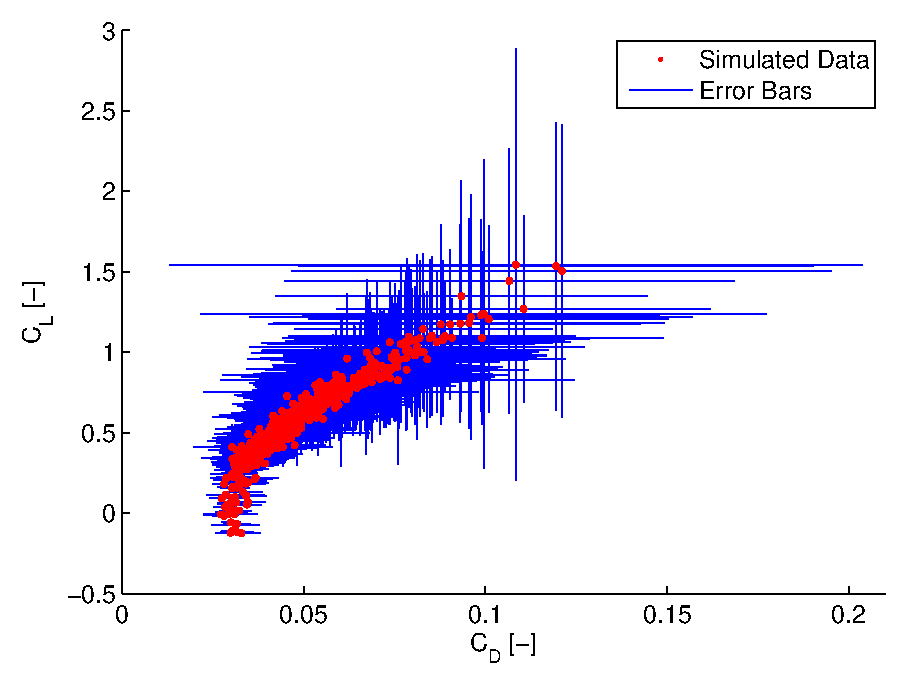
\includegraphics[width=0.5\textwidth]{figures/heteroskedasticity.eps}
      \caption{Heteroskedastic Error from Simulated Flight}
      \label{fig:errorBars}
\end{figure}


%todo:cite the fact that heteroskedasticity does not color the estimate
While heteroskedasticity does not color the estimate of $\hat{\beta}_i$, it does color the confidence intervals. The method of dealing with this problem is discussed in the next section.


\section*{Least Squares Regression Error}
The error of a single data point is not the main driving factor in the accuracy of a regression model. The important factor in the model is how accurately the coefficients are known, which is a function of the accuracy of each point, as well as the number of points sampled. The main parameter that describes the accuracy of the regression coefficients are the confidence intervals. A confidence interval is a range of values such that, if the experiment were repeated, the parameter calculated would be within the range some percentage of the time. A parameter can be represented as an estimated value, with a confidence bound

\begin{align}
\label{confidenceInterval}
\beta &= \beta_{EST} \pm t\frac{\sigma}{\sqrt{n}}
\end{align}

where $\beta$ is the parameter in question, $\beta_{EST}$ is the estimated value of the parameter, $t$ is the Student's $t$ value based on the number of samples and the desired confidence interval, $\sigma$ is the standard deviation of the sample, and $n$ is the number of data points collected. Since the number of data points collected during flight will be large ($n>100$), the $t$ value will be taken as 1.96 for a 95\% confidence interval.\\
As previously mentioned, one of the assumptions made in a Least Squares regression is homoskedasticity. However, the error using standard uncertainty propagation is heteroskedastic. This becomes a problem in estimating confidence intervals, because the standard error can be driven by outliers. If each data point had the same error, these outliers could be valid. However, if the data is heteroskedastic, the outlier may have larger error bounds (see Figure \ref{fig:errorBars},) meaning the data point is not as likely as it first appears. This fact can drive the standard error estimate to be larger than is appropriate, which leads to a larger confidence interval and possibly a false lack of rejection of the confidence interval's hypothesis test. To account for this, the \texttt{robustfit} function in MATLAB  was used to estimate both the coefficients and robust standard error estimates. The \texttt{robustfit} function calculates heteroskedastically-robust standard error estimates by doing a weighted average, where the weighting is based on a radial basis function. This means that the farther away a data point is from the estimated regression model, the less impact it has on the standard error of the model. The default weighting function used by \texttt{robustfit} is bisquare, and it was used for this research.

\section*{Kalman Filter Regression Error}
Kalman filters are often used to propagate states. The filter does this by combining the system dynamics with a measured state. The variance is propagated using Equation \ref{kalmanVariance}. When estimating coefficients using the Kalman filter, the $\bar{A}$ state transition matrix is an identity matrix, which is due to the fact that the coefficients stay constant. When propagated through the filter, this means the state estimate $x_k$ is essentially a variance-weighted-average of the coefficient estimates. The matrix $P_k$ contains the variance of the coefficient estimates. Equation \ref{confidenceInterval} calculates the confidence interval of regression coefficients and needs the standard deviation of the mean, also called the standard error. The matrix $P_k$ can be used  to calculate the confidence intervals by noting
\nomenclature{$\sigma$}{Standard deviation}
\begin{align}
\bar{P}_k &= \begin{bmatrix}
\sigma_{1}^2 &  0  & \ldots & 0\\
0  &  \sigma_{2}^2 & \ldots & 0\\
\vdots & \vdots & \ddots & \vdots\\
0  &   0       &\ldots & \sigma_i^2
\end{bmatrix}
\end{align}

The confidence interval for coefficient $\beta_i$ can be calculated using $\sigma_i$ in Equation \ref{confidenceInterval}.
